\chapter{Reactive Streams}\label{reactive-streams}

\begin{quote}
Reactive Streams is an initiative to provide a standard for asynchronous
stream processing with non-blocking back pressure. This encompasses
efforts aimed at runtime environments (JVM and JavaScript) as well as
network protocols.
\end{quote}

The project is a collaboration between engineers from Kaazing, Netflix,
Pivotal, RedHat, Twitter, Typesafe and many others and is developed and
discussed in the open.

The core idea behind the Reactive Stream standard is in the definition
of two different channels for the \textbf{downstream data} and the
\textbf{upstream demand}.

\begin{figure}[htbp]
\centering

\includegraphics[scale=0.25]{imgs/stream.png}
\caption{Two different channels for the downstream data and the upstream
demand}
\end{figure}

This allows overcoming one of the biggest issue of the Rx approaches:
\textbf{backpressure}. Backpressure is a lack of demand, and is due to
the fact that the producer of a stream of items is faster than the
consumer, and that difference of speed quickly determines a growing
backlog of unconsumed items on the consumer side.

In the literature (and in our everyday life) there's already a protocol
that solved a similar problem: TCP. With this in mind, engineers behind
Reactive Streams proposed a solution that, in simple terms, works like
this:

\begin{itemize}
\itemsep1pt\parskip0pt\parsep0pt
\item
  A publisher doesn't send data until a request arrives via the demand
  channel, at which point it can push a certain number of elements (in
  according to the request) downstream.
\item
  When outstanding demand exists, the publisher is free to push data to
  the subscriber.
\item
  When demand is exhausted, the publisher cannot send data except as a
  response to demand signalled from downstream.
\end{itemize}

Engineers called this technique \textbf{dynamic push/pull}. The dynamic
terms indicates that the system should \textbf{adapt} to the current
conditions of its components and that's not safe to only use a
\emph{just push} or just \emph{pull approach}.

A \textbf{just push} approach is not safe when the \textbf{subscriber is
slow}, since it'll quickly start to be overwhelmed by the offers and
will start to:

\begin{itemize}
\itemsep1pt\parskip0pt\parsep0pt
\item
  drop items, in the case of it use a bounded buffer to store received
  messages (just like TCP)
\item
  trigger an out of memory error
\end{itemize}

A \textbf{just pull} approach is too slow in the case that the
\textbf{subscriber is faster} than the publisher.

Two important notes about the fact that data and demand \emph{flows} in
different channels and directions are the following:

\begin{itemize}
\itemsep1pt\parskip0pt\parsep0pt
\item
  \textbf{Merging streams splits the upstream demand}
\item
  \textbf{Splitting streams merges the downstream demand}
\end{itemize}

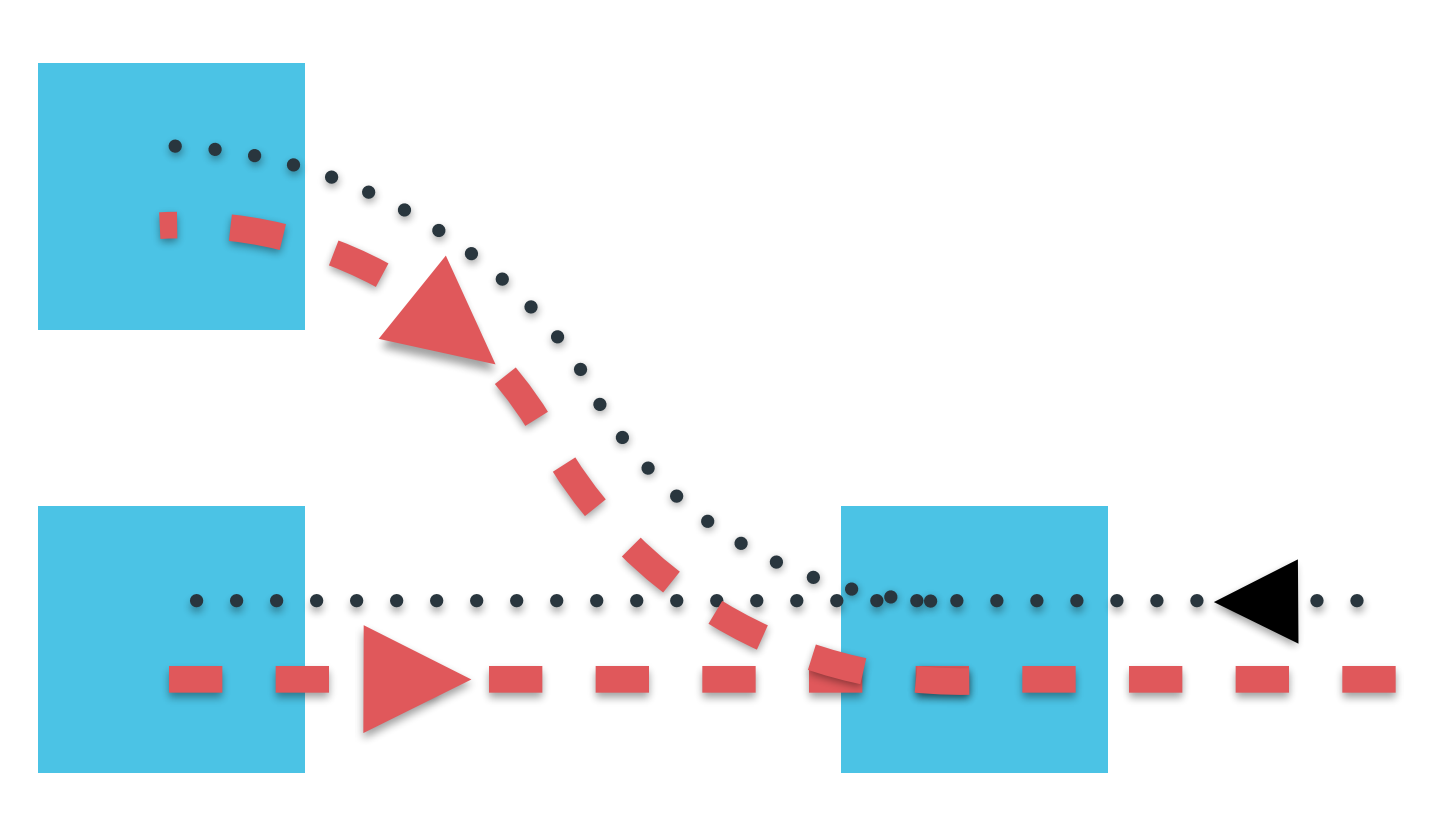
\includegraphics[scale=0.25]{imgs/merge.png} 
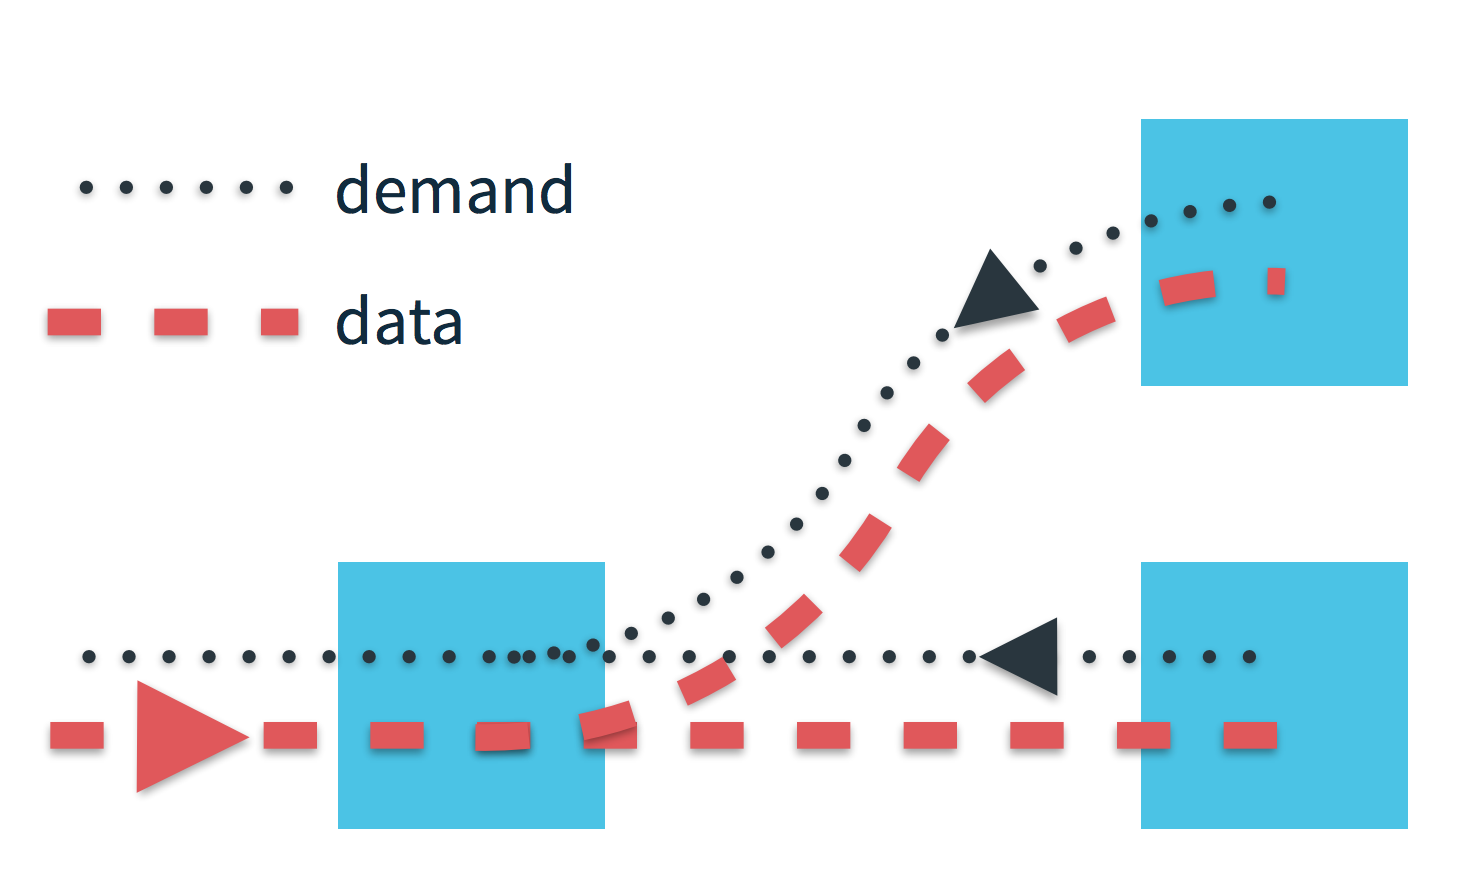
\includegraphics[scale=0.25]{imgs/split.png}

As the main document says, the scope of Reactive Streams is to find a
minimal set of interfaces, methods and protocols that will describe the
necessary operations and entities to achieve the goal: asynchronous
streams of data with non-blocking back pressure. This set of interfaces
is a low level specification to which each library should conform.

The API offers the following interfaces that are required to be
implemented by each implementation:

\begin{itemize}
\itemsep1pt\parskip0pt\parsep0pt
\item
  Subscriber
\item
  Subscription
\item
  Publisher
\item
  Processor
\end{itemize}


\section{Subscriber}\label{subscriber}

The \textbf{Subscriber} interface abstracts the notion of an entity that
consumes items. Its definition is as follows.

\begin{verbatim}
public interface Subscriber<T> {
    public void onSubscribe(Subscription s);
    public void onNext(T t);
    public void onError(Throwable t);
    public void onComplete();
}
\end{verbatim}

A \texttt{Subscriber} has the canonical \texttt{onNext(\ )},
\texttt{onError(\ )}, and \texttt{onComplete()} methods. When new items
are produced by the publisher, a the onNext method is invoked with the
new element. If an error was raised while producing values, the
publisher would then invoke the onError method with the exception.
Finally, when the publisher completes its job, the onComplete method is
then invoked.

The \texttt{onSubscribe(\ )} method is invoked when a subscriber is
subscribed to a publisher. This method is really important for the
framework, since it links the relation between a subscriber and a
publisher, via a \texttt{Subscription}.

\section{Subscription}\label{subscription}

A \textbf{Subscription} abstracts the notion of a subscriber's
communication channel back to the publisher. This channel is what
enables the subscriber to either cancel the subscription or signal
demand. Its definition is as follows.

\begin{verbatim}
public interface Subscription {
    public void request(long n);
    public void cancel();
}
\end{verbatim}

The \texttt{request(\ )} method signals to the publisher that the
subscriber can receive more items, also specifying the quantity.

The \texttt{cancel(\ )} method notifies the publisher that the
subscriber is no longer interested in receiving items.

This channel between a publisher and a subscriber is what enables to
achieve non blocking back-pressure in a Reactive Streams.

\section{Publisher}\label{publisher}

The \textbf{Publisher} interface has only one method to implement, and
is as follows.

\begin{verbatim}
public interface Publisher<T> {
    public void subscribe(Subscriber<? super T> s);
}
\end{verbatim}

A subscriber is subscribed to a publisher via the \texttt{subscribe(\ )}
method. This method doesn't return a \texttt{Subscription} as one would
expect, but \texttt{Unit}. This is a precise design choice, since every
method of the interfaces returns \texttt{Unit}.

The publisher, after notifying the subscriber that it has been
subscribed via its \texttt{onSubscribed(\ )} method, must provide items
to the subscriber, that will receive items in its \texttt{onNext(\ )}
method. The items received must not exceed the total number of items
that the subscriber has signalled demand for.

When the subscriber \texttt{cancel(\ )} the subscription, the publisher
must start sending items.

Finally, a publisher must notify to the subscriber through
\texttt{onError(\ )} and \texttt{onComplete(\ )} methods if an error is
encountered or the stream is successfully completed respectively.

\section{Processor}\label{processor}

A \textbf{Processor} represents a processing stage, which is both a
Subscriber and a Publisher and obeys the contracts of both. The
interface is defined as follows.

\begin{verbatim}
public interface Processor<T, R>
    extends Subscriber<T>, Publisher<R> { }
\end{verbatim}

A processor is an intermediate abstraction that enables to build
\textbf{chain of processing stage}, in which each intermediate unit is a
processor that can consume, transform and publish items. The importance
of this abstraction is in the fact that, obeying to both Subscriber and
Publisher interface, it has to \textbf{retain back-pressure
propagation} with the original stream source.



